% Åbo Akademi University nonofficial LaTeX-tempate for PhD-theses
% Contributed by Andreas Lundell, Anders Skjäl, Jan Kronqvist and others

\documentclass[10pt, b5paper]{memoir}
% *************** Document style definitions ***************

% *************** Load packages ***************

%\usepackage[english,swedish]{babel}
\usepackage[english]{babel}

\usepackage{microtype}

% Used for generating dummy text, can be removed
\usepackage{blindtext}

\usepackage{graphicx}
\usepackage{amsmath}
\usepackage{amssymb}
\usepackage{amsthm}

% Defines the fonts
\usepackage[]{kpfonts}
\usepackage[T1]{fontenc}

\usepackage{tikz}
\usetikzlibrary{shapes,arrows,positioning}
\usepackage{pgfplots}

% Used to include the papers
\usepackage{pdfpages}

\usepackage[small,bf]{caption}


% ************** Included papers ***************

% For creating the numbering between included papers 
\newcommand{\articlenumbering}[2]{
\cleardoublepage
\thispagestyle{empty}
\begin{tikzpicture}[remember picture, overlay]
	\node [shift={(-4 cm, #2)}]  at (current page.north east)
  {
	\begin{tikzpicture}[remember picture, overlay]
    \draw[fill=black] (0,0) rectangle (4,3);
		\node[draw=none,color=white] at (2.1,1.47) {\fontsize{25mm}{30mm}\selectfont #1};
	\end{tikzpicture}
	};
\end{tikzpicture}
\cleardoublepage
}

% For the bibliography
%\usepackage[numbers, sort&compress]{natbib}
\usepackage[square, comma, sort&compress]{natbib}

% Defines special mathematical operators

%\def\sgn{\mathop{\text{sgn}}}
%\def\rad{\mathop{\text{rad}}}
%\def\mid{\mathop{\text{mid}}}
%\def\diag{\mathop{\text{diag}}}
%\def\conc{\text{conc}}
%\def\conv{\text{conv}}
%\def\argmin{\mathop{\text{argmin}}}

%\newcommand{\vect}[1]{\boldsymbol{#1}}


% *************** Chapter and section style ***************

% Uncomment for alternative style for chapter headings
%\chapterstyle{veelo} 

\newcommand{\chaptertitle}[1]{#1}
\newcommand{\setchaptertitle}[1]{\renewcommand{\chaptertitle}{#1}}
\makepagestyle{mypagestyle}

% For verso pages
\makeevenhead{mypagestyle}{\thepage}{}{\slshape CHAPTER \thechapter}

% For recto pages
\makeoddhead{mypagestyle}{\slshape\MakeUppercase \chaptertitle}{}{\thepage}

% Activate your new pagestyle
\pagestyle{mypagestyle}

% *************** Page layout ***************

\settypeblocksize{*}{32pc}{1.618}
\settrimmedsize{250mm}{176mm}{*}
\setlrmargins{*}{20mm}{*}
%\setulmargins{27mm}{22mm}{*}
\setulmarginsandblock{27mm}{22mm}{*}
\setheadfoot{\onelineskip}{2\onelineskip}
\setheaderspaces{*}{2\onelineskip}{*}
\def\baselinestretch{1.1}

\checkandfixthelayout

% *************** Numbering ***************

\numberwithin{equation}{chapter}
%\numberwithin{equation}{section}

\numberwithin{figure}{chapter}
\numberwithin{table}{chapter}

% *************** Defines theorems, etc. ***************

%\newtheorem{theorem}{Theorem} % for numbering 1,2,3
\newtheorem{theorem}{Theorem}[chapter] % for numbering 1.1,1.2
%\newtheorem{theorem}{Theorem}[section] % for numbering 1.1.1,1.2.1

\newtheorem{corollary}[theorem]{Corollary}
\newtheorem{lemma}[theorem]{Lemma}
\newtheorem{proposition}[theorem]{Proposition}
\newtheorem{question}[theorem]{Question}
\theoremstyle{definition}
\newtheorem{definition}[theorem]{Definition}
\newtheorem{example}[theorem]{Example}
\newtheorem{remark}[theorem]{Remark}

% *************** End of document style definition ***************


\begin{document}

% *************** Front matter ***************
\frontmatter
% *************** Front matter ***************

% ***************************************************
% You should specify the contents of title page here
% Then you can specify dedication page or disable it
% ***************************************************

% *************** Title page ***************
\thispagestyle{empty}

\begin{center}
    \Huge
    
    \noindent The very long and very difficult thesis title should go here
    
    \vfill
    \vfill
    
    \LARGE
    \noindent Firstname Lastname
    
    \vfill
    \vfill
    
    
\includegraphics[width=0.38\textwidth]{sigill.png}
    %0.4
    
    \vfill
    
    \large
    
    \noindent
    PhD Thesis in Mathematics\\
    Mathematics and Statistics\\
    Faculty of Science and Engineering\\
    {\AA}bo Akademi University\\
    \vfill
    {\AA}bo, Finland 2019

\end{center}

% Creates page with IBAN numbers

\clearpage
\thispagestyle{empty}

\null\vfill

\begin{center}
   
	978-952-12-3749-2 \\
    978-952-12-3750-8 (pdf)\\
	\vspace{5mm}
	Painosalama Oy\\
	{\AA}bo 2018
\end{center}

\clearpage

% Creates the dedication page
\chapter*{Preface}
\addcontentsline{toc}{chapter}{Preface}%

Dedication to all the people that has helped with the thesis comes here...

\Blindtext[2]

\vspace{2cm}
{\AA}bo, January 2019

\vspace{1cm}
Firstname Lastname
	
\cleardoublepage

% Includes the summary in Swedish
\chapter*{Svensk sammanfattning}
\addcontentsline{toc}{chapter}{Svensk sammanfattning}%

\blindmathtrue
\Blindtext[4]
\blindmathfalse

\cleardoublepage

% Creates the table of contents and list of figures and tables if needed

\tableofcontents
%\clearpage
%\listoffigures
%\clearpage
%\listoftables

% *************** End of front matter ***************

% *************** Main matter ***************
\mainmatter

% It is easier to create a seperate tex-file for each chapter and then include them here

\chapter{Introduction}

\blindmathtrue
\Blindtext

\section{List of publications}

The thesis is based on the following publications. Some text about the authors contributions to the publications should be made here.

\begin{description}
\item[\textbf{Paper I}] F.~Lastname, F.~Lastname and F.~Lastname, \emph{Title of the paper here}, Journal Name, pp. 1-100, 2019. DOI:~ 10.1007/s00605-018-1216-5
\item[\textbf{Paper II}] F.~Lastname, F.~Lastname and F.~Lastname, \emph{Title of the paper here}, Journal Name, pp. 1-100, 2019. DOI:~ 10.1007/s00605-018-1216-5
\item[\textbf{Paper III}] F.~Lastname, F.~Lastname and F.~Lastname, \emph{Title of the paper here}, Journal Name, pp. 1-100, 2019. DOI:~ 10.1007/s00605-018-1216-5
\item[\textbf{Paper IV}] F.~Lastname, F.~Lastname and F.~Lastname, \emph{Title of the paper here}, Journal Name, pp. 1-100, 2019. DOI:~ 10.1007/s00605-018-1216-5
\end{description}





\chapter{Some preliminaries}

A citation to \cite{lundell2009transformation} and \cite{lundell2009some} for the sake of illustration.

\begin{definition}
    A definition can be used to define things.
\end{definition}

\begin{theorem}
    Here is a theorem with proof with an equation
        \begin{equation}
            a+b=c.
        \end{equation}
\end{theorem}

\begin{proof}
Test
\end{proof}

\begin{lemma}
    A lemma.
\end{lemma}

\begin{remark}
    A remark.
\end{remark}

\begin{example}
    Here is also an example.
\end{example}

\blindmathfalse
\Blindtext

\begin{figure}[t]
    \centering
    
\includegraphics[width=4cm]{sigill.png}
    \caption{This is the official seal of {\AA}bo Akademi University.}
    \label{fig:my_figure}
\end{figure}

\Blindtext

\begin{figure}[tb]
    \centering
    \begin{tikzpicture}
    	\begin{axis}[
    		xlabel=$x$,
    		ylabel={$f(x) = x^2 - x +4$}
    	]
    	% use TeX as calculator:
    	\addplot {x^2 - x +4};
    	\end{axis}
    \end{tikzpicture}
    \caption{Use \texttt{pgfplots} for simple and not so simple plots.}
    \label{fig:my_plot}
\end{figure}

\Blindtext


\begin{table}[t]
    \centering
    \begin{tabular}{ l c r }
      1 & 2 & 3 \\
      4 & 5 & 6 \\
      7 & 8 & 9 \\
    \end{tabular}
    \caption{This is a table.}
    \label{fig:my_table}
\end{table}



\blindmathtrue
\Blinddocument


% *************** Bibliography ***************
%\bibliographystyle{unsrt} % for numbering within brackets
\bibliographystyle{plainnat} % for author-year

\bibliography{bibliography}

% *************** Appendixes ***************
%\appendix
%\appendixpage*
%\input{app1/app1.tex}


% *************** Articles ***************

% Remember to compile LaTeX twice to get everything working

% Change the path to the included files and remember to update the roman numbering for each
\articlenumbering{I}{-7cm}
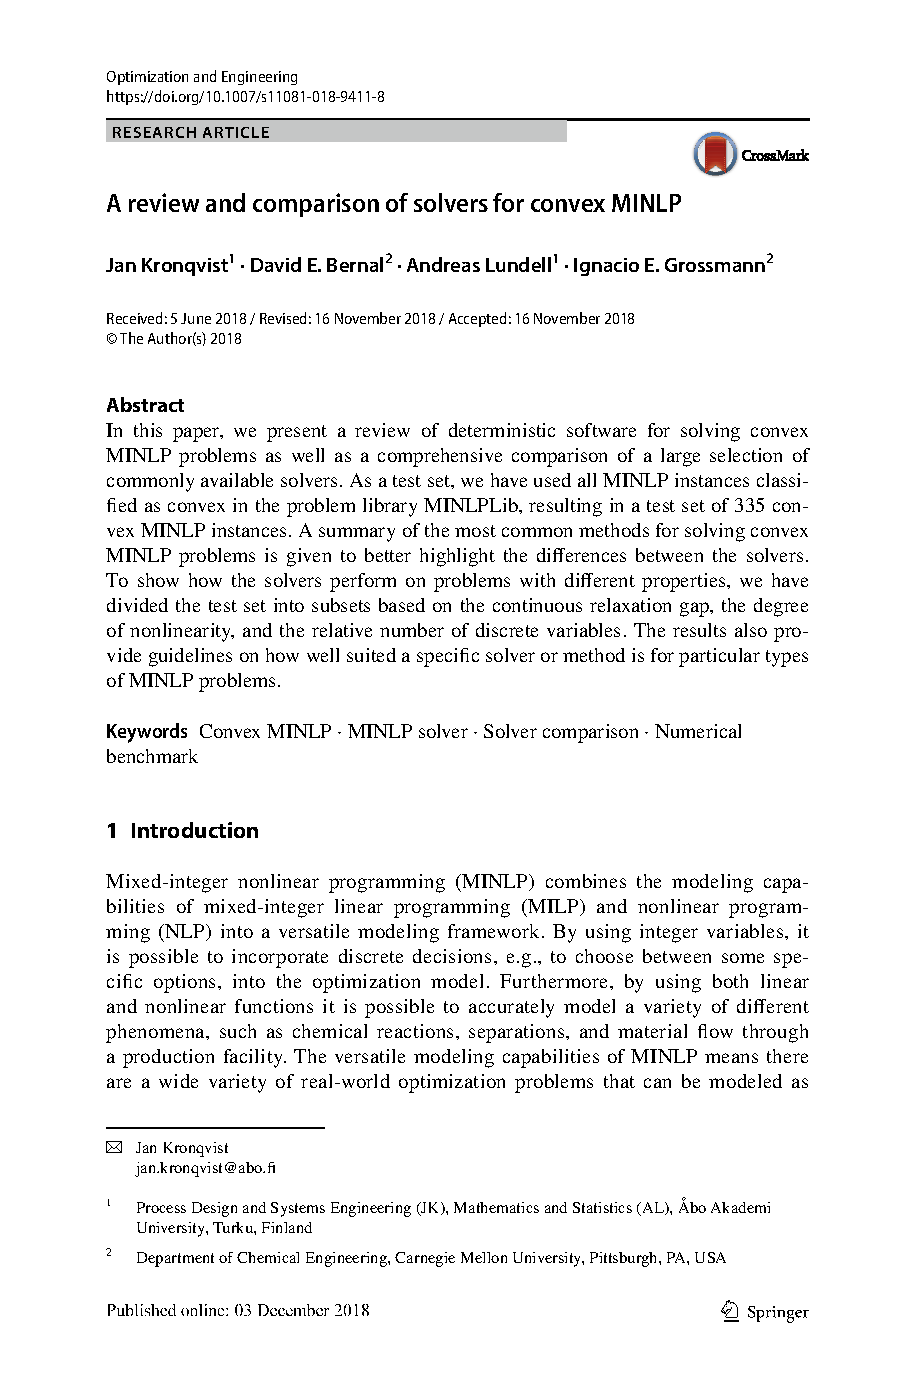
\includepdf[pages={1-}]{papers/paper1.pdf}

\end{document}